\chapter{حركة الأغشية وفرز البروتينات}\label{ch:b3:membrane-traffic}

تصنع خلية من البنكرياس نحو عشرة ملايين جزيء من الإنزيم الهاضم
في الدقيقة، وتحزمها في حبيبات، وتطلقها في
قناة عند إشارة من الأمعاء --- من غير أن تطلق قط جزيء
تربسين واحدًا في هيولاها. وتأخذ خلية كبدية الكوليسترول من
الدم بابتلاع الجسيمات التي تحمله، كاملةً، بمعدل
آلاف في الدقيقة، وتعيد كل مستقبل إلى السطح
للجسيم التالي. والبروتين المصنوع حديثًا المقدَّر للمتقدرة، أو
للنواة، أو \omterm{def:b3:membrane-traffic:endocytosis}{للجسيم الحال}، أو للغشاء، أو للعالم الخارجي يبلغ عنوانه
بين عشرات المقصورات بمعدل خطأ يخجل منه
البريد. وهذا الفصل عن الفرز: الإشارات
المكتوبة في البروتينات، والآلات التي تقرؤها، والحويصلات التي
تحمل الغشاء والحمولة بين المقصورات، والمعاطف التي تشكّل
الحويصلات والبروتينات التي تجعلها تندمج بالهدف الصحيح، و
الحركة في الاتجاهين --- إفراز إلى الخارج، والتقام إلى الداخل --- التي
تواصلها الخلية حقيقية النواة كل ثانية من حياتها.

\section{الإشارات والعناوين}

\begin{definition}[إشارات الفرز]\label{def:b3:membrane-traffic:signals}
\index{إشارة فرز}\index{ببتيد إشارة}\index{إشارة التوطين النووي}\index{تسلسل أمامي}
\emph{إشارة الفرز} قطعة من بروتين، أو تعديل
فيه، يقرؤها مستقبل يوصل البروتين إلى مقصورة واحدة.
و\emph{ببتيد الإشارة} شوط من \numrange{15}{30} بقية عند
النهاية الأمينية له لبّ كاره للماء، يرسل البروتين إلى
الشبكة الهيولية الباطنة وهو يُصنع؛ ومن هناك يقود الطريق الافتراضي
عبر \omterm{prop:b3:membrane-traffic:golgi}{جهاز غولجي} إلى الغشاء الهيولي أو إلى الخارج،
وتحوّله إشارات أخرى إلى \omterm{def:b3:membrane-traffic:endocytosis}{الجسيم الحال} (سكر مفسفر) أو
رجوعًا إلى الشبكة (التسلسل الكربوكسيلي الطرفي KDEL). و
\emph{إشارة التوطين النووي}، وهي رقعة قاعدية قصيرة مثل
PKKKRKV، ترتبط بها إمبورتينات تحمل البروتين المطوي عبر
المسام النووي؛ و\emph{التسلسل الأمامي} المتقدري، وهو
لولب برمائي من \numrange{20}{50} بقية، تتعرفه مستقبلات على
الغشاء الخارجي ويُمرَّر، غير مطوي، عبر ناقلات الغشاءين؛
وإنزيمات البيروكسيسوم تنتهي بالتسلسل SKL. والبروتينات التي لا شيء من هذه فيها
تبقى في العصارة الخلوية. وقد وُجدت كل إشارة بالطريقة نفسها: فحذفها
يترك البروتين في العصارة، وتطعيمها على بروتين عصاري
يرسل ذلك البروتين إلى المقصورة.
\end{definition}

\begin{proof}[شواهد]
ترجم بلوبل ودوبرشتاين (1975) RNA الرسول لسلسلة خفيفة من جسم
مضاد في منظومة خالية من الخلايا. فمن دون أغشية كان
الناتج أطول بنحو عشرين بقية من البروتين المفرَز؛
ومع إضافة قطع من الشبكة الهيولية الباطنة \emph{أثناء} الترجمة،
كان للناتج حجم البروتين المفرَز وكان محميًا من البروتياز
المضاف --- إذ كان داخل الحويصلات --- في حين لم تفعل الأغشية المضافة
بعد الترجمة شيئًا. فالقطعة الأمينية الطرفية الزائدة، وهي
\omterm{def:b3:membrane-traffic:signals}{ببتيد الإشارة}، لازمة لدخول الشبكة، وتُزال داخلها،
ولا تعمل إلا والسلسلة تُصنع: وهي \emph{فرضية
الإشارة}، التي تأكدت في كل تفصيل حين نُقّي المستقبل (وهو
جسيم التعرف على الإشارة، والتر وبلوبل 1981) والقناة
(Sec61).
\end{proof}

\begin{omfigure}
\begin{tikzpicture}[every node/.style={font=\scriptsize}, >=stealth]
  % ER membrane
  \fill[omDef!15] (0,0) rectangle (12,-1.6);
  \draw[very thick, omDef] (0,0) -- (12,0); \draw[very thick, omDef] (0,-0.35) -- (12,-0.35);
  \node[right, omDef!70!black] at (0.1,-1.3) {لمعة الشبكة};
  \node[right] at (0.1,2.9) {العصارة الخلوية};
  % stage 1: ribosome with emerging signal peptide + SRP
  \draw[thick, fill=gray!25] (1.4,1.6) circle (0.5); \draw[thick, fill=gray!25] (1.4,0.95) ellipse (0.62 and 0.3);
  \draw[very thick, omThm] (1.4,0.65) -- (1.4,0.2) -- (1.9,0.1);
  \draw[thick, fill=omProp!40] (2.1,0.35) ellipse (0.35 and 0.2); \node[above right] at (2.2,0.5) {SRP};
  \node[below, align=center] at (1.7,-1.7) {1. يبرز ببتيد الإشارة؛\\يرتبط SRP، وتتوقف الترجمة};
  % stage 2: docking at SRP receptor and translocon
  \draw[->, thick] (3.2,1.2) -- (4.2,1.2);
  \draw[thick, fill=gray!25] (5.6,1.75) circle (0.5); \draw[thick, fill=gray!25] (5.6,1.1) ellipse (0.62 and 0.3);
  \draw[thick, fill=omMeth!40] (5.2,0.0) rectangle (5.45,-0.35); \draw[thick, fill=omMeth!40] (5.75,0.0) rectangle (6.0,-0.35);
  \node[below, align=center] at (5.9,-1.7) {2. يرسو مستقبل SRP الريبوزوم\\على Sec61؛ ويغادر SRP};
  \draw[very thick, omThm] (5.6,0.8) -- (5.6,-0.2);
  \draw[thick, fill=omProp!40] (4.7,0.15) ellipse (0.3 and 0.18); \node[above] at (4.7,0.33) {مستقبل SRP};
  % stage 3: translocation, cleavage, glycosylation
  \draw[->, thick] (7.2,1.2) -- (8.2,1.2);
  \draw[thick, fill=gray!25] (9.6,1.75) circle (0.5); \draw[thick, fill=gray!25] (9.6,1.1) ellipse (0.62 and 0.3);
  \draw[thick, fill=omMeth!40] (9.2,0.0) rectangle (9.45,-0.35); \draw[thick, fill=omMeth!40] (9.75,0.0) rectangle (10.0,-0.35);
  \draw[very thick, omThm] (9.6,0.8) -- (9.6,-0.5) .. controls (9.6,-1.0) and (10.3,-1.1) .. (10.6,-0.7);
  \draw[omThm, thick] (10.9,-0.9) -- (11.2,-0.9); \node[right, font=\tiny] at (11.0,-1.15) {قُطعت الإشارة};
  \fill[omExo] (10.3,-1.0) circle (0.07); \fill[omExo] (10.45,-1.12) circle (0.07); \node[below, font=\tiny] at (10.2,-1.15) {سكريات};
  \node[below, align=center] at (10.0,-1.7) {3. تعبر السلسلة وهي تُصنع؛\\تُقطع الإشارة، وتُضاف السكريات};
\end{tikzpicture}

{\small فرضية الإشارة. \omterm{def:b3:membrane-traffic:signals}{ببتيد الإشارة} عند بداية السلسلة
الوليدة يرتبط به جسيم التعرف على الإشارة، فيوقف
الترجمة ويرسي الريبوزوم على قناة Sec61؛ ثم تعبر السلسلة
الغشاء وهي تُركَّب، وتُقطع الإشارة في
اللمعة، وتُضاف السكريات.}
\end{omfigure}

\begin{proposition}[البروتينات الغشائية وطوبولوجيتها]\label{prop:b3:membrane-traffic:topology}
\index{تسلسل إيقاف النقل}\index{طوبولوجيا الغشاء}
الشوط الكاره للماء من نحو عشرين بقية في وسط
سلسلة تُنقل يعمل تسلسلَ \emph{إيقاف نقل}: فتنفتح
القناة جانبيًا وتطلقه في الطبقة الثنائية لولبًا
عابرًا للغشاء، ويبقى ما نُقل من قبل في اللمعة
وما بقي يُصنع نحو العصارة. والشوط الثاني من هذا القبيل يعيد بدء
النقل، والبروتين الذي فيه $n$ إشارة متناوبة ينتهي وفيه
$n$ لولبًا عابرًا للغشاء. والاتجاه المضبوط في الشبكة
لا يتغير أبدًا: فما يواجه لمعة الشبكة يواجه لمعة
غولجي ولمعة كل حويصلة بعدها، ويواجه \emph{خارج}
الخلية بعد الاندماج بالغشاء الهيولي. ومن ثم تكون السكريات، المضافة في
اللمعة وحدها، على الوجه خارج الخلوي من بروتين سطحي دائمًا،
ويمكن قراءة طوبولوجيا مستقبل من موضع مواقع غلكزته.
\end{proposition}

\begin{method}[النبض والملاحقة]\label{met:b3:membrane-traffic:pulse-chase}
\index{النبض والملاحقة}\index{تصوير إشعاعي ذاتي}
لمتابعة جمهرة من الجزيئات المصنوعة حديثًا عبر الخلية: (1)
عرّض الخلايا وقتًا قصيرًا (\emph{النبضة}، بضع دقائق) إلى
طليعة مشعة أو موسومة على نحو آخر --- كالليوسين المُثرَّت
للبروتينات؛ (2) استبدل بها فائضًا من طليعة غير موسومة (
\emph{الملاحقة})، فلا يُدخل واسم جديد؛ (3) ثبّت عينات من
الخلايا على فترات وحدّد موضع الواسم \omterm{met:b3:membrane-traffic:pulse-chase}{بالتصوير الإشعاعي الذاتي} في الصور
المجهرية الإلكترونية، أو بعزل المقصورات والعدّ؛ (4) ارسم
نسبة الواسم في كل مقصورة في مقابل الزمن. فترتيب امتلاء
المقصورات وتفريغها هو الطريق؛ والتوقيت يعطي
زمن المكث في كل منها. وطبّقه مختبر بالادي (في ستينيات القرن العشرين) على
خلية البنكرياس العنبية فوجد الواسم في الشبكة الخشنة عند
\qty{3}{min}، وفي غولجي عند \qty{20}{min}، وفي الفجوات المكثِّفة و
الحبيبات عند \qty{40}{min}، وفي القناة بعد ساعة وعلى
إشارة: أي المسلك الإفرازي، مبسوطًا في الزمن.
\end{method}

\begin{theorem}[المقصورات المتعاقبة ومنحنيات النبض والملاحقة]\label{thm:b3:membrane-traffic:pulse-chase}
\index{نموذج المقصورات}
لتغادر نبضة من بروتين موسوم المقصورةَ $A$ إلى $B$ بمعدل
من الرتبة الأولى $k_{1}$ ولتغادر $B$ إلى $C$ بمعدل $k_{2}$، مع احتفاظ
$C$ به. وبوجود الواسم كله في $A$ عند $t = 0$،
\[
A(t) = e^{-k_{1}t},\qquad
B(t) = \frac{k_{1}}{k_{2} - k_{1}}\bigl(e^{-k_{1}t} - e^{-k_{2}t}\bigr),
\qquad
C(t) = 1 - A - B,
\]
ويبلغ الواسم في $B$ ذروته عند $t^{*} = \ln(k_{2}/k_{1})/(k_{2} - k_{1})$.
وزمن المكث الوسطي في $A$ هو $1/k_{1}$ وفي $B$ هو $1/k_{2}$،
أيًا كان ترتيب المعدلين.
\end{theorem}
\begin{proof}
$\mathrm{d}A/\mathrm{d}t = -k_{1}A$ تعطي الأسّي. وأما $B$ فلدينا
$\mathrm{d}B/\mathrm{d}t = k_{1}A - k_{2}B = k_{1}e^{-k_{1}t} - k_{2}B$؛
فجرّب $B = \beta(e^{-k_{1}t} - e^{-k_{2}t})$: فمشتقته
$\beta(-k_{1}e^{-k_{1}t} + k_{2}e^{-k_{2}t})$ و$-k_{2}B = \beta(-k_{2}
e^{-k_{1}t} + k_{2}e^{-k_{2}t})$، فتقتضي المعادلة $\beta(k_{2}
- k_{1})e^{-k_{1}t} = k_{1}e^{-k_{1}t}$، أي $\beta = k_{1}/(k_{2} -
k_{1})$، و$B(0) = 0$ كما هو مطلوب. وبوضع $\mathrm{d}B/\mathrm{d}t =
0$: $k_{1}e^{-k_{1}t} = k_{2}e^{-k_{2}t}$، ومنها $t^{*}$. والزمن الوسطي
الذي يقضيه جزيء في مقصورة يغادرها بمعدل $k$ هو $\int_{0}^{
\infty} t\,k e^{-kt}\,\mathrm{d}t = 1/k$.
\end{proof}

\begin{example}[خلية بالادي بالأرقام]\label{ex:b3:membrane-traffic:palade}
خذ $k_{1} = \qty{0.1}{min^{-1}}$ (أي عشر دقائق في الشبكة) و
$k_{2} = \qty{0.05}{min^{-1}}$ (وعشرين في غولجي). فيبلغ غولجي ذروته عند
$t^{*} = \ln 2/0.05 = \qty{13.9}{min}$، ويحمل عندها $B = 2(e^{-1.39} -
e^{-0.69}) = 2(0.25 - 0.50)\cdot(-1) = 0.50$: أي نصف الواسم. وعند
\qty{40}{min}، $A = 0.018$، و$B = 2(0.018 - 0.135) \to 0.23$، و$C = 0.75$:
أي بلغت ثلاثةُ أرباع البروتين الحبيبات. ومنحنيات
مختبر بالادي المرصودة لها هذا الشكل، ومطابقتها كانت
أول قياس لأزمنة المكث.
\end{example}

\begin{omfigure}
\begin{tikzpicture}
\begin{axis}[
  width=0.7\linewidth, height=5.6cm,
  axis x line=bottom, axis y line=left,
  xmin=0, xmax=80, ymin=0, ymax=1.05,
  xlabel={الدقائق بعد النبضة}, ylabel={نسبة الواسم},
  xlabel style={font=\small, at={(axis description cs:0.5,-0.12)}, anchor=north},
  ylabel style={font=\small},
  tick label style={font=\small}, xtick={0,20,40,60,80}, ytick={0,0.5,1},
  clip=false,
]
\addplot[very thick, omDef, domain=0:80, samples=80] {exp(-0.1*x)};
\addplot[very thick, omProp, domain=0:80, samples=80] {2*(exp(-0.05*x)-exp(-0.1*x))};
\addplot[very thick, omMeth!70!black, domain=0:80, samples=80] {1-exp(-0.1*x)-2*(exp(-0.05*x)-exp(-0.1*x))};
\node[font=\scriptsize, omDef, anchor=south west] at (axis cs:4,0.62) {الشبكة، $A$};
\node[font=\scriptsize, omProp, anchor=south] at (axis cs:14,0.53) {غولجي، $B$};
\node[font=\scriptsize, omMeth!70!black, anchor=north west] at (axis cs:45,0.72) {الحبيبات، $C$};
\end{axis}
\end{tikzpicture}

{\small منحنيات \omterm{met:b3:membrane-traffic:pulse-chase}{النبض والملاحقة} من نموذج المعدلين عند $k_{1} =
\qty{0.1}{min^{-1}}$ و$k_{2} = \qty{0.05}{min^{-1}}$: يغادر الواسم
الشبكة أسّيًا، ويمر بغولجي بذروة عند
\qty{14}{min}، ويتراكم في الحبيبات.}
\end{omfigure}

\section{الشبكة الهيولية الباطنة: الطي والسكريات والجودة}

\begin{definition}[الغلكزة بالنتروجين ومراقبة الجودة]\label{def:b3:membrane-traffic:glycosylation}
\index{غلكزة بالنتروجين}\index{دورة الكالنكسين}\index{تحلل مرتبط بالشبكة}\index{استجابة البروتينات غير المطوية}
حين تدخل السلسلة اللمعةَ يُنقل قليل سكريد مجمَّع سلفًا من
أربعة عشر سكرًا (اثنان من N-أستيل غلوكوزامين، وتسعة مانوزات، وثلاثة
غلوكوزات) من حامل دهني إلى أسباراجينات في
التسلسل Asn-X-Ser/Thr --- وهي \emph{الغلكزة بالنتروجين}. ثم تُقلّم
الغلوكوزات الثلاثة واحدًا واحدًا، والتقليم ساعةُ طي:
فالبروتين الذي ما يزال يحمل غلوكوزًا واحدًا يمسكه المرافق الكالنكسين؛
والبروتين الذي أُزيل غلوكوزه الأخير وهو لم ينطوِ
بعد تعيد إنزيمة غلكزته، وهي تتعرف الرقع الكارهة للماء
المكشوفة، فيعود إلى الكالنكسين --- وهي \emph{دورة
الكالنكسين}. أما البروتينات التي تخفق مرارًا فتُسحب رجوعًا إلى العصارة،
وتُؤبقن ويهدمها البروتيازوم: وهو \emph{التحلل المرتبط
بالشبكة} (ERAD). وحين تتراكم البروتينات غير المطوية أسرع مما
يمكن طيّها أو هدمها، تطلق مستشعرات في غشاء الشبكة
\emph{استجابة البروتينات غير المطوية}: فتبطؤ الترجمة، و
تُحرَّض مورّثات المرافقات، وتتوسع الشبكة، وإذا دام الكرب
قُتلت الخلية. وأشيع طفرات التليف الكيسي
($\Delta$F508 في CFTR) تصنع قناة كانت لتعمل لكنها تنطوي ببطء
شديد، فيلتقطها ERAD ولا تبلغ السطح؛ والأدوية التي
تعينها على الطي صارت اليوم علاجًا.
\end{definition}

\begin{omfigure}
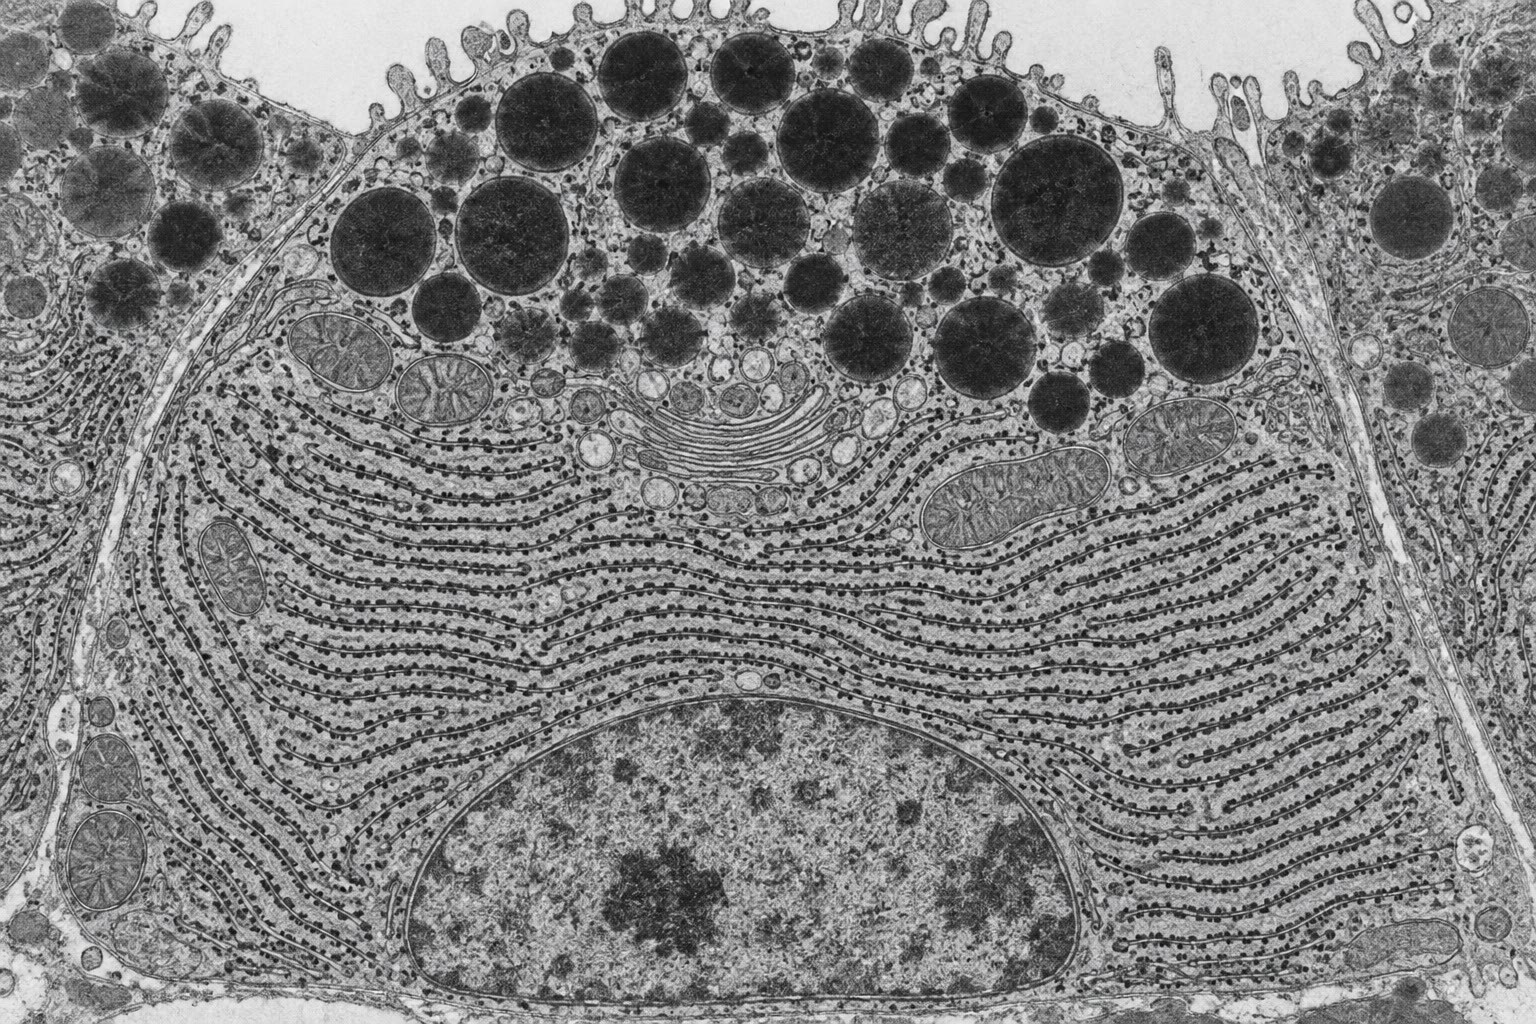
\includegraphics[width=0.56\linewidth]{images/book5/ai/b5-08-pancreas-acinar.jpg}

{\small خلية بنكرياسية عنبية في المجهر الإلكتروني: شبكة هيولية باطنة
خشنة مرصوفة مرصّعة بالريبوزومات تملأ القاعدة،
ويقع غولجي فوق النواة، وتُحزَم حبيبات إفرازية كثيفة من
الإنزيم الهاضم تحت السطح القمي، تنتظر
إشارة.}
\end{omfigure}

\section{الحويصلات: التبرعم والاستهداف والاندماج}

\begin{definition}[المعاطف وتبرعم الحويصلات]\label{def:b3:membrane-traffic:coats}
\index{حويصلة مغطاة}\index{COPII}\index{COPI}\index{كلاذرين}\index{GTPase صغير}
يشكّل الحويصلةَ الناقلة \emph{معطف} من البروتينات يتجمع على
الوجه العصاري لغشاء، فيحني الغشاء برعمًا
قطره \qtyrange{60}{100}{nm}، ويجمع الحمولة بمستقبلات تعبر
الغشاء، ويُنبذ بعد انفصال الحويصلة. وثلاثة معاطف
تخدم الطرق الرئيسة: \emph{COPII} للحويصلات المغادرة الشبكةَ
إلى غولجي، و\emph{COPI} لحركة العودة من غولجي إلى
الشبكة وبين صهاريج غولجي، و\emph{الكلاذرين} --- وهو
بروتين ثلاثي الأرجل يتبلمر في قفص من سداسيات
وخماسيات --- للحويصلات المغادرة غولجي البعيد إلى الجسيمات الداخلية و
للالتقام عند الغشاء الهيولي، حيث تربط بروتينات المهايئ
القفص بالمستقبلات المُدخَلة. ويستقدم كلَّ معطف
\emph{GTPase صغير} (وهو Sar1 مع COPII، وArf1 مع COPI والكلاذرين) يندس
في الغشاء في صورته المرتبطة بجزيء GTP، ويدع المعطف يسقط عند حلمهة GTP بعد
التبرعم. وتبقي إشاراتُ الاسترجاع المقصوراتِ
متمايزة: فبروتينات الشبكة الهاربة الحاملة KDEL يرتبط بها في
غولجي مستقبل ويعيدها في حويصلات COPI.
\end{definition}

\begin{omfigure}
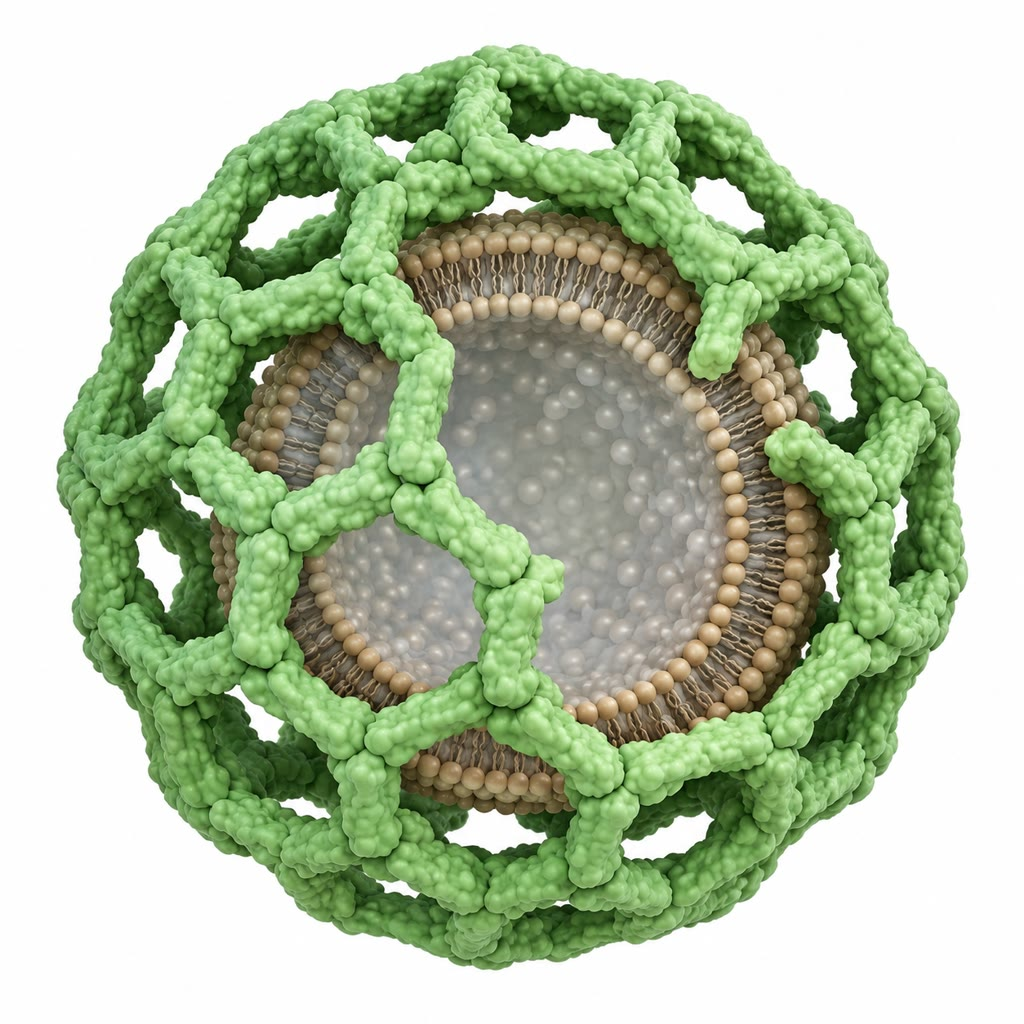
\includegraphics[width=0.36\linewidth]{images/book5/ai/b5-08-clathrin-cage.jpg}\hspace{0.04\linewidth}
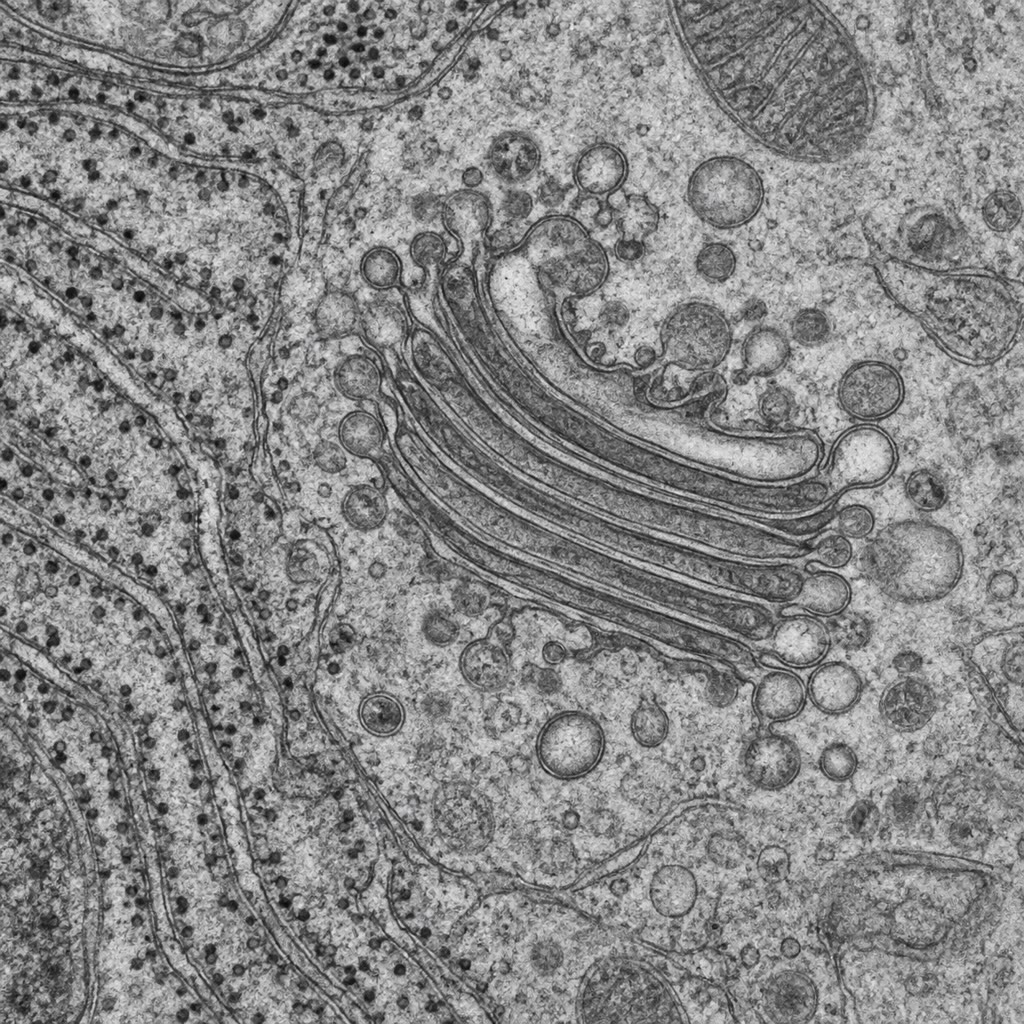
\includegraphics[width=0.36\linewidth]{images/book5/ai/b5-08-golgi-tem.jpg}

{\small يسارًا: قفص \omterm{def:b3:membrane-traffic:coats}{كلاذرين}، وهو الشبيكة متعددة الوجوه من وحدات
ثلاثية الأرجل تشكّل حويصلة التقام (مقطوعة لإظهار الغشاء
في داخلها). يمينًا: رصة غولجي في المجهر الإلكتروني، وهي كومة من
صهاريج مسطحة تتبرعم منها حويصلات عند الحواف.}
\end{omfigure}

\begin{definition}[الاستهداف والاندماج]\label{def:b3:membrane-traffic:fusion}
\index{GTPase من نمط Rab}\index{SNARE}\index{اندماج الأغشية}\index{سينابتوتاغمين}
تجد الحويصلة هدفها بطبقتين من التعرف. أولاهما \emph{إنزيمات
Rab من نمط GTPase} --- وهي نحو ستين في الخلية البشرية، كل منها على أغشية
مقصورة واحدة --- تستقدم بروتينات مِربَط طويلة تلتقط حويصلة
قادمة تحمل Rab الموافق. ثم تعمل \emph{بروتينات SNARE}: إذ يلتف
v-SNARE على الحويصلة وt-SNARE على الهدف، وهي بروتينات لولبية
مثبتة في غشاءيها، تلتف بعضها حول بعض من نهاياتها
القاصية نحو الغشاءين، فتشد طاقةُ حزمة اللوالب الأربعة التي
تكوّنها الطبقتين الثنائيتين حتى تندمجا. وكل ازدواج SNARE
نوعي، وهو فحص ثانٍ للعنوان. وبعد الاندماج تُفكَّك الحزمة
بإنزيم NSF من نمط ATPase لإعادة الاستعمال. ويمكن أن يُجعل الاندماج ينتظر
إشارة: ففي النهاية العصبية تُمسك بروتينات SNARE نصف مسحوبة
بالكومبلكسين حتى يتم \emph{السينابتوتاغمين}، بارتباطه بالكالسيوم الداخل حين
يصل كمون عمل، السحبَ في أقل من
مليثانية --- وهو إطلاق الناقل العصبي المتناوَل في كتاب السنة~الثانية.
وذيفانا الكزاز والتسمم الوشيقي بروتيازان يقطعان
بروتينات SNARE.
\end{definition}

\begin{proof}[شواهد]
عزل نوفيك وشيكمان (1980) طافرات خميرة حساسة للحرارة
تكفّ عن الإفراز عند \qty{37}{\celsius} وتراكم
البروتين في أي مقصورة يحجبها عيبها --- الشبكة،
أو غولجي، أو حويصلات مكوّمة تحت السطح؛ وحددت مورّثات \emph{sec} البالغة $23$
الخطوات، ثم تبيّن بعد استنساخها أنها تشفّر المعاطف و
إنزيمات GTPase وبروتينات \omterm{def:b3:membrane-traffic:fusion}{SNARE}. وأعاد روثمان تركيب النقل بين صهاريج
غولجي في أنبوب اختبار بأغشية منقّاة وعصارة وATP،
ونقّى منه NSF وبروتينات \omterm{def:b3:membrane-traffic:fusion}{SNARE}؛ فتلاقى المسلكان
على البروتينات نفسها، وتبيّن أن آلة الخميرة وآلة الثدييات
واحدة.
\end{proof}

\begin{omfigure}
\begin{tikzpicture}[every node/.style={font=\scriptsize}, >=stealth]
  % three stages left to right
  \foreach \x/\gap/\lab in {0/1.2/{1. يربطها Rab}, 4.4/0.55/{2. تلتف بروتينات SNARE}, 8.8/0.0/{3. اندماج، وإطلاق الحمولة}} {
    % target membrane
    \draw[very thick, omDef] (\x,0) -- (\x+3.4,0); \draw[very thick, omDef] (\x,-0.3) -- (\x+3.4,-0.3);
    \node[below, align=center] at (\x+1.7,-0.45) {\lab};
  }
  % stage 1 vesicle
  \draw[very thick, omProp] (1.7,1.2+0.8) circle (0.8); \draw[very thick, omProp] (1.7,1.2+0.8) circle (0.6);
  \draw[omThm, thick] (1.4,1.25) -- (1.4,0.35); \draw[omThm, thick] (2.0,1.25) -- (2.0,0.35);
  \draw[omMeth!70!black, thick] (1.7,1.2) -- (1.7,0.6); \draw[omMeth!70!black, thick] (1.7,0.6) -- (1.7,0.0);
  \draw[thick, fill=omExo!40] (0.7,0.9) ellipse (0.25 and 0.2); \node[left] at (0.45,0.9) {Rab};
  \draw[thick, omExo!70!black] (0.95,0.9) .. controls (1.1,0.5) .. (1.2,0.05); \node[left, font=\tiny] at (0.9,0.4) {مِربَط};
  \node[right, font=\tiny] at (2.05,0.8) {بروتينات SNARE};
  % stage 2 vesicle closer, helices twisted
  \draw[very thick, omProp] (6.1,0.55+0.8) circle (0.8); \draw[very thick, omProp] (6.1,0.55+0.8) circle (0.6);
  \draw[omThm, very thick] (5.85,0.6) .. controls (6.2,0.5) and (5.9,0.3) .. (6.1,0.05);
  \draw[omMeth!70!black, very thick] (6.35,0.6) .. controls (6.0,0.5) and (6.3,0.3) .. (6.1,0.05);
  \node[right, font=\tiny, align=left] at (6.6,0.35) {حزمة اللوالب الأربعة\\تشد الغشاءين\\معًا};
  % stage 3 fused omega shape
  \draw[very thick, omProp] (9.7,0) .. controls (9.7,1.5) and (11.3,1.5) .. (11.3,0);
  \draw[very thick, omProp] (9.9,-0.3) .. controls (9.9,1.1) and (11.1,1.1) .. (11.1,-0.3);
  \foreach \p in {(10.5,-0.9),(10.2,-1.1),(10.8,-1.15)} \fill[omExo] \p circle (0.06);
  \draw[->, omExo, thick] (10.5,0.5) -- (10.5,-0.6);
  \node[right, font=\tiny, align=left] at (11.4,0.8) {ثم يفكّ NSF\\بروتينات\\SNARE};
\end{tikzpicture}

{\small الاندماج في ثلاث خطوات. يقرّب Rab على الحويصلة ومِربَط على
الهدف الغشاءين حتى يتلامسا؛ ثم تلتف بروتينات \omterm{def:b3:membrane-traffic:fusion}{SNARE} في الحويصلة وفي الهدف
(بالأحمر والأخضر) في حزمة من أربعة لوالب تجرّ
الطبقتين الثنائيتين معًا؛ فتندمجان وتدخل الحمولة المقصورةَ
الهدف.}
\end{omfigure}

\begin{proposition}[جهاز غولجي]\label{prop:b3:membrane-traffic:golgi}
\index{جهاز غولجي}\index{نضج الصهاريج}\index{مانوز-6-فوسفات}
غولجي رصة من أربعة إلى ثمانية صهاريج مسطحة، وجهها القريب
نحو الشبكة ووجهها البعيد نحو الغشاء الهيولي، ويؤوي كل
صهريج طقمًا مختلفًا من الإنزيمات تقلّم سكريات البروتينات
السكرية المارة وتعيد بناءها وتضيف سكريات مرتبطة بالأكسجين وكبريتًا و
فوسفاتًا. وتتقدم الحمولة أساسًا عبر \emph{\omterm{prop:b3:membrane-traffic:golgi}{نضج الصهاريج}}: إذ يتكوّن
صهريج جديد عند الوجه القريب من حويصلات قادمة، ويتحرك عبر
الرصة كما فعلت التي سبقته، وينضج إذ تحمل حويصلات \omterm{def:b3:membrane-traffic:coats}{COPI}
إنزيمات كل صهريج رجوعًا إلى الأصغر الذي خلفه؛ وعند
الوجه البعيد يتفكك إلى حويصلات متجهة إلى مقاصدها.
وهناك يُقرَّر الفرز: فالحلمهات الجسيمية الحالة، الموسومة في غولجي
القريب بجزيء \emph{مانوز-6-فوسفات}، يرتبط بها مستقبلها وتُحزم
في حويصلات \omterm{def:b3:membrane-traffic:coats}{كلاذرين} إلى \omterm{def:b3:membrane-traffic:endocytosis}{الجسيم الداخلي}؛ والبروتينات الإفرازية المنظَّمة
تتكتل عند pH الحمضي الخفيف في حبيبات مكثِّفة؛
وكل ما عداها يغادر في التيار البنيوي إلى السطح. وفي
داء الخلايا I ينقص الإنزيم المفسفِر، فتُفرَز الحلمهات
بدل أن توصَّل، وتمتلئ الجسيمات الحالة بالمواد
غير المهضومة.
\end{proposition}

\begin{omfigure}
\begin{tikzpicture}[every node/.style={font=\scriptsize}, >=stealth]
  % plasma membrane top
  \draw[very thick, omDef] (0,4.2) -- (12,4.2); \node[above] at (6,4.25) {الغشاء الهيولي \quad (الخارج أعلاه)};
  % ER
  \draw[thick, fill=omDef!12] (0.3,0.0) rectangle (4.0,0.9); \node at (2.15,0.45) {الشبكة الهيولية الباطنة};
  % Golgi stack
  \foreach \y in {1.5,1.85,2.2,2.55} \draw[thick, fill=omProp!25] (4.8,\y) ellipse (1.4 and 0.13);
  \node[right] at (6.3,1.5) {قريب}; \node[left] at (3.35,2.55) {بعيد};
  \node[right] at (6.3,2.05) {رصة غولجي};
  % ER -> Golgi (COPII)
  \draw[->, thick, omMeth!70!black] (3.9,0.95) -- (4.5,1.4); \node[right, omMeth!70!black, font=\tiny] at (4.35,1.02) {COPII};
  % Golgi -> ER (COPI)
  \draw[->, thick, omThm] (3.6,1.42) -- (2.9,0.95); \node[left, omThm, font=\tiny] at (2.95,1.3) {COPI، استرجاع KDEL};
  % trans Golgi -> PM constitutive
  \draw[->, thick, omMeth!70!black] (5.6,2.7) -- (7.6,4.1); \node[left, font=\tiny, align=right] at (6.4,3.6) {إفراز\\بنيوي};
  % trans -> secretory granule -> PM regulated
  \draw[->, thick, omMeth!70!black] (4.6,2.7) -- (4.0,3.3); \draw[thick, fill=omExo!50] (3.8,3.5) circle (0.22); \draw[->, thick, omMeth!70!black] (3.8,3.75) -- (3.8,4.1);
  \node[left, font=\tiny, align=right] at (3.55,3.5) {حبيبة إفرازية:\\منظَّمة، على إشارة};
  % trans -> endosome/lysosome (clathrin, M6P)
  \draw[->, thick, omProp!80!black] (6.0,2.62) -- (8.25,2.62); \node[above, font=\tiny] at (7.1,2.67) {كلاذرين، مستقبل M6P};
  \draw[thick, fill=omProp!20] (8.8,2.7) circle (0.5); \node at (8.8,2.7) {\tiny جسيم داخلي};
  \draw[->, thick, omProp!80!black] (9.25,2.4) -- (10.2,1.95); \draw[thick, fill=omThm!25] (10.7,1.6) circle (0.5); \node at (10.7,1.6) {\tiny جسيم حال};
  % endocytosis from PM to endosome
  \draw[->, thick, omDef] (9.6,4.15) -- (9.1,3.2); \node[right, font=\tiny, align=left] at (9.5,3.7) {التقام\\(حفر كلاذرين)};
  % recycling endosome -> PM
  \draw[->, thick, omDef] (8.5,3.2) -- (8.0,4.15); \node[left, font=\tiny] at (8.3,3.3) {إعادة تدوير};
  % lysosome inputs autophagy
  \draw[->, thick, gray] (11.9,0.6) -- (11.1,1.3); \node[below, font=\tiny, align=center] at (11.9,0.55) {جسيم التهام ذاتي\\(هيولى، عضيّات)};
\end{tikzpicture}

{\small خريطة حركة الأغشية. إلى الخارج (بالأخضر): من الشبكة إلى غولجي
في حويصلات \omterm{def:b3:membrane-traffic:coats}{COPII}، ومن غولجي إلى السطح إما بنيويًا وإما عبر
حبيبات تنتظر إشارة. وإلى الوراء (بالأحمر): تعيد حويصلات \omterm{def:b3:membrane-traffic:coats}{COPI}
بروتينات الشبكة الهاربة. وإلى الأسفل (بالبرتقالي): الإنزيمات الجسيمية الحالة الموسومة بجزيء
مانوز-6-فوسفات تذهب إلى \omterm{def:b3:membrane-traffic:endocytosis}{الجسيم الداخلي} \omterm{def:b3:membrane-traffic:endocytosis}{والجسيم الحال}. وإلى الداخل (بالأزرق):
التقام من السطح، مع إعادة تدوير معظم المستقبلات.}
\end{omfigure}

\section{الالتقام والجسيم الحال}

\begin{definition}[الالتقام]\label{def:b3:membrane-traffic:endocytosis}
\index{التقام بوساطة المستقبلات}\index{جسيم داخلي}\index{جسيم حال}\index{التهام ذاتي}
\emph{الالتقام بوساطة المستقبلات} يركّز رابطةً مرتبطة
بمستقبلات سطحية في حفر مغطاة \omterm{def:b3:membrane-traffic:coats}{بالكلاذرين}، تنفصل (إذ يضيّق
إنزيم دينامين من نمط GTPase العنق) حويصلاتٍ قطرها نحو \qty{100}{nm}
--- أي ألف في الدقيقة في خلية ليفية، فيدور غشاء السطح
كله في ساعة. وتندمج الحويصلات في \emph{جسيمات داخلية
باكرة} تُحمَّض لمعتها إلى pH~6 بمضخة بروتونات؛ ومعظم
الربائط تطلق مستقبلاتها هناك، فتعود المستقبلات إلى
السطح في حويصلات إعادة تدوير، وتمضي الرابطة مع نضج
الجسيم الداخلي إلى جسيم داخلي متأخر (pH~5.5) واندماجه مع
\emph{جسيم حال}: وهو مقصورة عند pH~4.5--5 تحوي نحو ستين
حلمهة --- بروتيازات، ونوكليازات، ولبيازات، وغليكوزيدازات --- لا تنشط
إلا عند ذلك pH، فلا يضر تسربها إلى العصارة المتعادلة
كثيرًا. ويهضم الجسيم الحال أيضًا مواد الخلية نفسها الموصَّلة عبر
\emph{الالتهام الذاتي}: إذ ينمو غشاء مزدوج حول جزء من الهيولى
أو حول عضيّة بالية، وينغلق جسيمَ التهام ذاتي، ويندمج
بالجسيم الحال؛ وتُعاد النواتج إلى العصارة. ويحرّض الالتهام الذاتي
الجوعُ (فهو يعيد تدوير مادة الخلية نفسها للطاقة)
وهو ينظّف التكتلات والمتقدرات المتأذية؛ ويُتهم إخفاقه
في التنكس العصبي.
\end{definition}

\begin{proof}[شواهد]
تابع براون وغولدشتاين (في سبعينيات القرن العشرين) البروتين الدهني منخفض الكثافة (LDL)،
وهو الجسيم الذي يحمل الكوليسترول في الدم، إلى خلايا ليفية
مزروعة. فارتبط LDL ارتباطًا قابلًا للإشباع بنحو \num{20000} موقع سطحي في
الخلية، وأُدخل في دقائق إلى حفر مغطاة، وأُطلق
كوليستروله في الجسيمات الحالة فأطفأ تركيب الخلية
للكوليسترول. أما الخلايا الليفية من مرضى فرط
كوليسترول الدم العائلي فلم تربط LDL (لغياب المستقبل) أو ربطته لكنها
لم تُدخله (لطفرة في ذيل المستقبل العصاري
تمنع التقاطه بمهايئات \omterm{def:b3:membrane-traffic:coats}{الكلاذرين}): فكان المرض
عيبًا في الالتقام، وكان ذيل المستقبل يحوي إشارة الإدخال،
وترسخ المستقبل المعاد تدويره --- وكل منه يقوم بمئات الجولات
--- آليةً عامة للالتقاط.
\end{proof}

\begin{proposition}[الالتقاط بمستقبلات معادة التدوير]\label{prop:b3:membrane-traffic:uptake}
\index{إعادة تدوير المستقبلات}
لتكن في خلية $R$ مستقبل جملةً، منها $S$ على السطح
و$R - S$ في الداخل في طريق العودة. والمستقبل السطحي مشغول
باحتمال $\theta = [L]/(K_{d} + [L])$، ويُدخَل المستقبل المشغول
بمعدل $k_{i}$، ويعود المستقبل المُدخَل بمعدل
$k_{r}$. وعند الحالة المستقرة يكون تدفق الرابطة إلى الخلية
\[
J = \frac{R\,k_{i}k_{r}\,\theta}{k_{r} + k_{i}\theta},
\]
وهو يتشبع، مع ارتفاع تركيز الرابطة، عند $J_{\max} =
R\,k_{i}k_{r}/(k_{i} + k_{r})$: فالتقاط الخلية لا تحدّه
مستقبلاتها وحدها بل سرعة إعادتها إياها.
\end{proposition}
\begin{proof}
تُفقد المستقبلات السطحية بمعدل $k_{i}\theta S$ وتُستعاد بمعدل
$k_{r}(R - S)$؛ وعند الحالة المستقرة يتوازنان، فتكون $S = R\,k_{r}/(k_{r}
+ k_{i}\theta)$. وكل إدخال يحمل رابطة واحدة، فتكون $J =
k_{i}\theta S$، وهي تعطي الصيغة. وحين $\theta \to 1$ يؤول التدفق
إلى $R\,k_{i}k_{r}/(k_{r} + k_{i})$ --- أي تدور المستقبلات بأسرع
ما يسمح به المعدلان، وتكون نسبة $k_{r}/(k_{i} + k_{r})$ منها
على السطح في أي لحظة.
\end{proof}

\begin{example}[الكوليسترول بالجسيم]\label{ex:b3:membrane-traffic:ldl}
الخلية الليفية ذات $R = \num{20000}$ مستقبل LDL، وزمن إدخال
قدره \qty{5}{min} ($k_{i} = \qty{0.2}{min^{-1}}$) وزمن عودة
قدره \qty{10}{min} ($k_{r} = \qty{0.1}{min^{-1}}$) تلتقط، عند LDL
المشبع، $J_{\max} = \num{20000}\times 0.2\times 0.1/0.3 \approx 1300$
جسيم في الدقيقة، مع ثلث مستقبلاتها على السطح في
أي لحظة؛ ويجلب كل جسيم نحو \num{1500} جزيء من
الكوليسترول، أي مليونين في الدقيقة، تكفي لبناء نحو عُشر
ميكرومتر مربع من الغشاء. أما متغاير اللواقح لفرط
كوليسترول الدم العائلي، وله نصف المستقبلات، فيلتقط نصف ذلك؛
فيتضاعف كوليسترول الدم، ويأتي داء القلب أبكر بعشرين سنة.
والستاتينات ترفع $R$ بتجويع الخلية الكبدية من كوليسترولها
هي.
\end{example}

\begin{omfigure}
\begin{tikzpicture}
\begin{axis}[
  width=0.7\linewidth, height=5.4cm,
  axis x line=bottom, axis y line=left,
  xmin=0, xmax=10, ymin=0, ymax=1500,
  xlabel={تركيز LDL، $[L]/K_{d}$}, ylabel={جسيمات في الدقيقة},
  xlabel style={font=\small, at={(axis description cs:0.5,-0.12)}, anchor=north},
  ylabel style={font=\small},
  tick label style={font=\small}, xtick={0,2,4,6,8,10}, ytick={0,500,1000,1333}, yticklabels={0,500,1000,$J_{\max}$},
  clip=false,
]
\addplot[very thick, omDef, domain=0:10, samples=60] {20000*0.2*0.1*(x/(1+x))/(0.1+0.2*(x/(1+x)))};
\addplot[very thick, omThm, domain=0:10, samples=60] {10000*0.2*0.1*(x/(1+x))/(0.1+0.2*(x/(1+x)))};
\addplot[dashed, gray, domain=0:10, samples=2] {1333};
\node[font=\scriptsize, omDef, anchor=north west] at (axis cs:4,900) {$R = \num{20000}$};
\node[font=\scriptsize, omThm, anchor=north west] at (axis cs:4,560) {$R = \num{10000}$ (متغاير اللواقح)};
\end{axis}
\end{tikzpicture}

{\small التقاط LDL بمستقبلات معادة التدوير، من صيغة
القضية عند $k_{i} = \qty{0.2}{min^{-1}}$ و$k_{r} =
\qty{0.1}{min^{-1}}$: وهو يتشبع بالرابطة، وينتصف حين ينقص نصف
المستقبلات.}
\end{omfigure}

\begin{remark}[غشاء واحد، مقصورات كثيرة]\label{rem:b3:membrane-traffic:one-membrane}
كل غشاء من المنظومة الإفرازية والالتقامية هو، طوبولوجيًا،
غشاء واحد: فلمعة الشبكة متصلة، عبر
الحويصلات، بخارج الخلية، ويستطيع دهن أو بروتين مصنوع في
الشبكة أن يبلغ السطح من غير أن يعبر طبقة ثنائية قط.
والذي يبقي المقصورات متمايزة ليس الجدران بل الحركة ---
حزم انتقائي إلى الخارج، واسترجاع انتقائي إلى الوراء، وزوج
نوعي من جزيئات التعرف عند كل اندماج. فالمقصورات حالات
مستقرة من التدفقات، مثل برك نهر، والخلية التي تتوقف عن
الحركة تفقد جغرافيتها في ساعات.
\end{remark}

\section{تمارين}

\begin{exercise}[$\star$]\label{exo:b3:membrane-traffic:1}
أعطِ الإشارة والمقصد لكل مما يلي: شوط من عشرين
بقية كارهة للماء عند النهاية الأمينية؛ وPKKKRKV؛ ولولب
برمائي أميني الطرف؛ وKDEL عند النهاية الكربوكسيلية؛ و
مانوز-6-فوسفات على السكريات.
\end{exercise}

\begin{exercise}[$\star$]\label{exo:b3:membrane-traffic:2}
صِف المشاهدات الثلاث الأساسية في تجربة بلوبل ودوبرشتاين
وما بيّنته كل منها.
\end{exercise}

\begin{exercise}[$\star$]\label{exo:b3:membrane-traffic:3}
سمِّ \omterm{def:b3:membrane-traffic:coats}{المعطف} واتجاه النقل في كل من: الشبكة إلى غولجي؛
وغولجي إلى الشبكة؛ وغولجي البعيد إلى \omterm{def:b3:membrane-traffic:endocytosis}{الجسيم الداخلي}؛ والغشاء الهيولي إلى
\omterm{def:b3:membrane-traffic:endocytosis}{الجسيم الداخلي}.
\end{exercise}

\begin{exercise}[$\star$]\label{exo:b3:membrane-traffic:4}
لماذا تكون سكريات بروتين الغشاء الهيولي على خارج
الخلية دائمًا؟
\end{exercise}

\begin{exercise}[$\star\star$]\label{exo:b3:membrane-traffic:5}
في نموذج \cref{thm:b3:membrane-traffic:pulse-chase} عند $k_{1}
= \qty{0.2}{min^{-1}}$ و$k_{2} = \qty{0.05}{min^{-1}}$، أوجد متى
يبلغ واسم غولجي ذروته وكم يكون فيه عند الذروة؛ ثم
نسبة ما في الحبيبات عند \qty{60}{min}.
\end{exercise}

\begin{exercise}[$\star\star$]\label{exo:b3:membrane-traffic:6}
بروتين غشائي فيه أشواط كارهة للماء من $22$ بقية عند
المواضع 30 و90 و150 و210 \omterm{def:b3:membrane-traffic:signals}{وببتيد إشارة} أميني الطرف.
ارسم أو صِف طوبولوجيته: كم لولبًا، وأي جانب تواجهه كل قطعة
بينها. وأين يمكن أن يُغلكز؟
\end{exercise}

\begin{exercise}[$\star\star$]\label{exo:b3:membrane-traffic:7}
باستعمال \cref{prop:b3:membrane-traffic:uptake} عند $R = \num{30000}$
و$k_{i} = \qty{0.25}{min^{-1}}$ و$k_{r} = \qty{0.05}{min^{-1}}$، احسب
$J_{\max}$ ونسبة المستقبلات على السطح عند الإشباع.
وأي تغير واحد يضاعف الالتقاط؟
\end{exercise}

\begin{exercise}[$\star\star$]\label{exo:b3:membrane-traffic:8}
تنبأ بمصير الحلمهات الجسيمية الحالة، وبالنمط الظاهري، في (أ)
خلية ينقصها مستقبل مانوز-6-فوسفات، و(ب) خلية ينقصها
الناقل الفوسفاتي الذي يضيف الوسم، و(ج) خلية معالَجة
بدواء يعادل pH \omterm{def:b3:membrane-traffic:endocytosis}{الجسيم الداخلي}.
\end{exercise}

\begin{exercise}[$\star\star$]\label{exo:b3:membrane-traffic:9}
طفرة JD في مستقبل LDL تبدّل تيروزينًا في الذيل
العصاري. فالخلايا تربط LDL طبيعيًا لكنها تخفق في التقاطه. فسّر
الآلية، وتنبأ بأين توجد المستقبلات على سطح الخلية
نسبةً إلى الحفر المغطاة.
\end{exercise}

\begin{exercise}[$\star\star\star$]\label{exo:b3:membrane-traffic:10}
حلّ نموذج \omterm{met:b3:membrane-traffic:pulse-chase}{النبض والملاحقة} في حالة $k_{1} = k_{2} = k$ (فصيغة
المبرهنة شاذة هناك): بيّن أن $B(t) = kt\,e^{-kt}$
وأوجد الذروة. ثم فسّر لماذا لا يستطيع قياس نسبة الحبيبات
$C(t)$ وحدها أن يحدد المعدلين كلًا على حدة.
\end{exercise}

\begin{exercise}[$\star\star\star$]\label{exo:b3:membrane-traffic:11}
خلية ليفية تُدخل \num{1000} حويصلة \omterm{def:b3:membrane-traffic:coats}{كلاذرين} قطرها \qty{100}{nm}
في الدقيقة وسطحها \qty{3000}{\micro m^2}. فكم
تستغرق إدخال ما يعادل السطح كله؟ ولماذا لا تنكمش
الخلية، وماذا يعني التوازن عن معدل
الإخراج الخلوي وعن حجم السائل الداخل في الساعة؟
\end{exercise}

\begin{exercise}[$\star\star\star$]\label{exo:b3:membrane-traffic:12}
ذيفان الوشيقية يقطع بروتين \omterm{def:b3:membrane-traffic:fusion}{SNARE} في النهايات العصبية الحركية؛ وذيفان
الكزاز يقطع البروتين نفسه في العصبونات البينية المثبطة في النخاع
الشوكي. فسّر لماذا يسبب الأول شللًا رخوًا والثاني شللًا
تشنجيًا، ولماذا يكون الذيفان الذي يحجب الاندماج نافعًا في الطب عند
جرعات ضئيلة.
\end{exercise}

\section{مسألة: يوم في حياة خلية بنكرياسية}

\begin{problem}[{مسألة نهاية الأسبوع --- إنتاجية خلية إفرازية
معدودةً بالجزيئات والحويصلات والميكرومترات المربعة، ومنحنيات
النبض والملاحقة فيها محلولة، والتقاط خلية كبدية للكوليسترول محسوبًا
بمستقبلات معادة التدوير، وجسيم حال محمَّض بروتونًا بروتونًا،
وتنتهي إلى زمن ذروة غولجي، والحويصلات المتبرعمة في الدقيقة
وجسيمات LDL الملتقَطة في الساعة}]
\label{pb:b3:membrane-traffic:1}
معطيات: خلية عنبية تصنع $10^{7}$ جزيء إنزيم في الدقيقة، كل منها
\qty{25}{kDa} وقطره \qty{4}{nm}. والحويصلات الناقلة كرات قطرها
\qty{70}{nm}؛ والحبيبة كرة قطرها \qty{1}{\micro m}.
ومساحة الغشاء لكل جزيء دهن \qty{0.7}{nm^2}، بطبقتين. و
مساحة شبكة الخلية \qty{6000}{\micro m^2}. \omterm{met:b3:membrane-traffic:pulse-chase}{والنبض والملاحقة}:
$k_{1} = \qty{0.1}{min^{-1}}$، و$k_{2} = \qty{0.05}{min^{-1}}$. وخلية
كبدية: $R = \num{50000}$ مستقبل LDL، و$k_{i} = \qty{0.2}{min^{-1}}$،
و$k_{r} = \qty{0.1}{min^{-1}}$، و$K_{d} = \qty{2}{nmol/L}$، وتركيز جسيمات
LDL في البلازما \qty{2}{nmol/L}؛ و\num{1500} جزيء كوليسترول
في الجسيم.
\omterm{def:b3:membrane-traffic:endocytosis}{وجسيم حال}: كرة قطرها \qty{0.5}{\micro m}، وpH من $7.2$ إلى $4.7$،
وسعة تنظيم حمضي تقتضي ضخّ $50$ بروتونًا لكل بروتون
يبقى حرًا؛ ومضخة البروتونات تنقل $200$ بروتون في الثانية.

\medskip
\noindent\textbf{الجزء الأول --- الإنتاجية.}
\begin{enumerate}
  \item ما كتلة الإنزيم التي تصنعها الخلية في الدقيقة، وفي اليوم؟
        قارنها بمحتوى الخلية نفسها من البروتين، وهو نحو
        \qty{300}{pg}.
  \item كم جزيء إنزيم يسع الحويصلة إذا ملأت
        \qty{30}{\%} من حجمها (وهي كرة قطرها \qty{4}{nm})؟ وكم
        حويصلة في الدقيقة تغادر الشبكة؟
  \item كم مساحة غشاء تحمل تلك الحويصلات في الدقيقة، و
        في كم من الزمن تستهلك الشبكة كلها لو لم يعد
        منها شيء؟
  \item كم جزيء دهن ذلك في الدقيقة؟ وما الذي يجب أن
        تفعله الخلية لتحفظ شبكتها؟
  \item كم جزيء إنزيم يسع الحبيبة عند الحزم نفسه،
        وكم حبيبة تملأ الخلية في الساعة؟
  \item وجبة تفرّغ $300$ حبيبة في عشر دقائق باندماجها
        بالغشاء القمي، فتضيف غشاءها إلى سطح قدره
        \qty{50}{\micro m^2}. بأي عامل ينمو السطح القمي،
        وما الذي يجب أن يتبع؟
\end{enumerate}

\medskip
\noindent\textbf{الجزء الثاني --- التوقيت.}
\begin{enumerate}[resume]
  \item بالمعدلات المعطاة، متى يبلغ واسم غولجي ذروته، وما
        النسبة التي فيه؟
  \item ما نسبة النبضة في الشبكة وغولجي و
        الحبيبات عند \qty{30}{min}؟
  \item أزمنة المكث الوسطية في المقصورتين؟ وما الزمن الكلي
        الوسطي من التركيب إلى الحبيبة؟
  \item دواء يبطئ الخروج من غولجي إلى $k_{2} = \qty{0.01}{min^{-1}}$.
        فما زمن الذروة الجديد ونسبتها؛ وكيف يبدو غولجي
        في المجهر؟
  \item فسّر لماذا تكون نسبة ذروة غولجي هي $k_{1}/k_{2}$ مرفوعة إلى
        أسّ (أعطِ الأسّ) ومن ثم تكون دائمًا دون $1$.
  \item لو كانت خطوة الشبكة أسرع بكثير من خطوة غولجي،
        فإلامَ تؤول $B(t)$؟ فسّر.
\end{enumerate}

\medskip
\noindent\textbf{الجزء الثالث --- الكوليسترول.}
\begin{enumerate}[resume]
  \item احسب $\theta$ عند تركيز LDL في البلازما، و
        الالتقاط $J$ بالجسيمات في الدقيقة وفي الساعة.
  \item كم جزيء كوليسترول في الساعة؟ وتحوي أغشية الخلية
        $5\times 10^{9}$ جزيء كوليسترول؛ فكم يلزم لاستبدالها
        كلها من LDL وحده؟
  \item احسب نسبة المستقبلات على السطح، وعدد
        الجولات التي يقوم بها كل مستقبل في عمره البالغ \qty{20}{h}.
  \item لمتغاير اللواقح $R = \num{25000}$: أعد حساب $J$. ويرتفع LDL
        البلازما حتى يطابق الالتقاطُ الإنتاجَ: فبأي عامل، إذا كانت
        $\theta$ دون الإشباع بكثير؟
  \item ستاتين يضاعف $R$ في خلايا كبد متغاير اللواقح. فماذا
        يحدث لجسيمات LDL في البلازما، بالتعليل نفسه؟
  \item فسّر لماذا يكون متماثل اللواقح عديم المستقبلات، وLDL بلازماه
        خمسة أضعاف السوي، أسوأ حالًا مما يوحي به حساب السؤال
        16 وحده.
\end{enumerate}

\medskip
\noindent\textbf{الجزء الرابع --- الحمض.}
\begin{enumerate}[resume]
  \item احسب حجم \omterm{def:b3:membrane-traffic:endocytosis}{الجسيم الحال} باللترات وعدد البروتونات
        الحرة عند pH $7.2$ وعند pH $4.7$.
  \item كم بروتونًا يجب ضخّه جملةً، مع التنظيم الحمضي؟
        وكم يستغرق ذلك بعدد $50$ مضخة؟
  \item تضخ المضخة البروتونات إلى الداخل ضد التدرج. فأي
        مشكلة كهربائية تنشأ، وكيف تُحلّ (فكّر في
        أيون مقابل)؟
  \item لماذا تُصنع الحلمهات فاعلةً عند pH~5 وحده، وما الذي يحميه
        ذلك؟
  \item لماذا يطلق مستقبل LDL جسيمَ LDL عند pH~6 بينما يطلق
        مستقبل مانوز-6-فوسفات حمولته عند pH نفسه ---
        وما الذي يجب أن يشترك فيه البروتينان؟
  \item الكلوروكين قاعدة ضعيفة تعبر الأغشية غير مشحونة
        وتُحتجز متى بُرتنت. فبأي عامل يتركز
        في \omterm{def:b3:membrane-traffic:endocytosis}{جسيم حال} عند pH $4.7$ نسبةً إلى العصارة عند
        pH $7.2$ (أي نسبة تركيزي البروتونات)، وماذا يفعل
        ذلك \omterm{def:b3:membrane-traffic:endocytosis}{بالجسيم الحال}؟
  \item لخّص: زمن ذروة غولجي (السؤال~7)، والحويصلات
        المغادرة الشبكةَ في الدقيقة (السؤال~2)، وجسيمات
        LDL الملتقَطة في الساعة (السؤال~13).
\end{enumerate}
\end{problem}
